%--------------------------------------------------------------------------------------%--------------------------------------------------------------------------------------
%
%  Global settings, dont change it! (excapt additional \usepackage commands)
%  Always use PDFLatex!
%
%--------------------------------------------------------------------------------------%--------------------------------------------------------------------------------------
\documentclass[a4paper, 12pt, oneside, BCOR1cm,toc=chapterentrywithdots]{scrbook}

\usepackage{graphicx}           % use for pdfLatex
\usepackage{makeidx} % f\"{u}r Benutzung des Befehls \printindex
\usepackage[colorlinks=false]{hyperref}
\usepackage{tocbibind}
\usepackage{blindtext}
\usepackage{subfigure}
\usepackage{acronym}
\usepackage{tikz}
\usetikzlibrary{arrows.meta,positioning,calc,patterns,fit}
\usepackage{amsmath}
\usepackage{array}
\usepackage{tabularx}
\newcolumntype{C}{>{\centering\arraybackslash}X} % centred, wrapping tabularx column

\hypersetup{%
bookmarksnumbered=true, hyperindex=true,
%
%Im Acrobat Reader Subtitel 1. Ebene anzeigen
bookmarksopen=true, bookmarksopenlevel=1,
%
pdfborder=0 0 0 % Keine Box um die Links!
}

% --------------------------------------------------------------
% Force Tables and List to be added in Table of Content
% --------------------------------------------------------------

\renewcommand*{\tableofcontents}{%
  	\begingroup
  	\tocsection
  	\tocfile{\contentsname}{toc}
  	\endgroup
}
\renewcommand*{\listoffigures}{%
  	\begingroup
  	\tocsection
  	\tocfile{\listfigurename}{lof}
  	\endgroup
}
\renewcommand{\listoftables}{
	\begingroup
	\tocsection
	\tocfile{\listtablename}{lot}
	\endgroup
}
\begin{document}

%--------------------------------------------------------------------------------------%--------------------------------------------------------------------------------------
%
%  Here starts the userspace !
%
%--------------------------------------------------------------------------------------%--------------------------------------------------------------------------------------

%--------titlepage
\begin{titlepage}

{
    \begin{center}
        \raisebox{-1ex}{
\includegraphics[scale=1.5]{TU_Chemnitz_positiv_gruen.pdf}}\\
    \end{center}
    \vspace{0.5cm}
}

\begin{center}

\LARGE{\textbf{Title of the master thesis}}\\
\vspace{1cm}


\Large{\textbf{Master Thesis}}\\ 
\vspace{1cm}
Submitted in Fulfilment of the\\
Requirements for the Academic Degree\\
M.Sc.\\
\vspace{0.5cm}
Dept. of Computer Science\\
Chair of Computer Engineering
\end{center}
\vspace{3cm}
Submitted by: Max Mustermann\\
Student ID: 111222\\
Date: 12.12.1212\\
\vspace{0.3cm}\\
Supervising tutor: Prof. Dr. W. Hardt \\
(further supervisors)

\end{titlepage}

%---------------------------------------------------------
% Abstract
%---------------------------------------------------------

\addchap*{Abstract}
\blindtext
\\\\
\textbf{Keywords: Keyword1, Keyword2, Keyword3, ...max 5}

%---------------------------------------------------------
% Table of Contents, List of figures, List of Tables
%---------------------------------------------------------

\tableofcontents
\listoffigures
\listoftables

%---------------------------------------------------------
% List of Abbreviations
%---------------------------------------------------------
\twocolumn
\addchap{List of Abbreviations}
\begin{acronym}[Bash]
 \acro{KDE}{K Desktop Environment}
 \acro{SQL}{Structured Query Language}
 \acro{Bash}{Bourne-again shell}
 \acro{JDK}{Java Development Kit}
 \acro{VM}{Virtuelle Maschine}
 \acro{I2C}[I²C]{Inter-Integrated Circuit}
 \acro{KDE}{K Desktop Environment}
 \acro{SQL}{Structured Query Language}
 \acro{Bash}{Bourne-again shell}
 \acro{JDK}{Java Development Kit}
 \acro{VM}{Virtuelle Maschine}
 \acro{I2C}[I²C]{Inter-Integrated Circuit}
 \acro{KDE}{K Desktop Environment}
 \acro{SQL}{Structured Query Language}
 \acro{Bash}{Bourne-again shell}
 \acro{JDK}{Java Development Kit}
 \acro{VM}{Virtuelle Maschine}
 \acro{I2C}[I²C]{Inter-Integrated Circuit}
 \acro{KDE}{K Desktop Environment}
 \acro{SQL}{Structured Query Language}
 \acro{Bash}{Bourne-again shell}
 \acro{JDK}{Java Development Kit}
 \acro{VM}{Virtuelle Maschine}
 \acro{I2C}[I²C]{Inter-Integrated Circuit}
 \acro{KDE}{K Desktop Environment}
 \acro{SQL}{Structured Query Language}
 \acro{Bash}{Bourne-again shell}
 \acro{JDK}{Java Development Kit}
 \acro{VM}{Virtuelle Maschine}
 \acro{I2C}[I²C]{Inter-Integrated Circuit}
 \acro{KDE}{K Desktop Environment}
 \acro{SQL}{Structured Query Language}
 \acro{Bash}{Bourne-again shell}
 \acro{JDK}{Java Development Kit}
 \acro{VM}{Virtuelle Maschine}
 \acro{I2C}[I²C]{Inter-Integrated Circuit}
\end{acronym}

\onecolumn
%---------------------------------------------------------
% Here starts the real work
%---------------------------------------------------------

\chapter{Introduction}
% just insert your text here

\blindtext[0]

\blindtext[4]

\blindtext[1]
  % Load Data from File intro.tex

\chapter{Background and State of the Art}
\label{ch:background}
% Chapter 2 -- to be written.

\chapter{Data Acquisition and Dataset Construction}
% Chapter 3 -- Data Acquisition and Dataset Construction
% Figures are authored in TikZ so the chapter compiles without external assets.
% Placeholders [VERIFY: ...] and [CITATION: ...] mark items still to be resolved.

\label{ch:data}

\tikzset{
  blk/.style={draw, rounded corners=2pt, align=center, inner sep=4pt,
              minimum height=8mm, font=\footnotesize},
  grp/.style={draw, dashed, rounded corners=3pt, inner sep=6pt},
  flow/.style={-{Latex[length=2mm]}, thick},
}

This chapter explains the process used to create the multimodal dataset used in
the remainder of this thesis. It introduces the wearable sensing platform and its
resource envelope, the assembly scenario, the activity classes recorded, the
firmware that streamed inertial and acoustic data off the devices, the protocol
used to record participants, the video-based annotation procedure, and the steps
of signal conditioning and windowing that transform the raw streams into labelled
two-second segments. The chapter ends with a quantitative characterisation of the
resulting dataset and an assessment of its known limitations. The modelling
choices made on this dataset are deferred to Chapter~\ref{ch:method}, and the
implications of the dataset's limitations for the validity of the results are
addressed in Chapter~\ref{ch:discussion}.

\section{Sensor Platform and Computational Constraints}
\label{sec:platform}

The sensing platform is the M5StickC Plus2, a self-contained wearable device built
around the ESP32-PICO-V3-02 system-on-chip (SoC), a dual-core processor clocked
up to 240\,MHz~\cite{m5stickcplus2}. Each device is equipped with a six-axis
inertial measurement unit (IMU, MPU6886) providing three-axis acceleration and
three-axis angular velocity, a digital MEMS microphone (SPM1423), a small
display, a single-cell 200\,mAh lithium-polymer battery, and a 2.4\,GHz Wi-Fi
radio~\cite{m5stickcplus2}.

\begin{figure}[!ht]
\centering
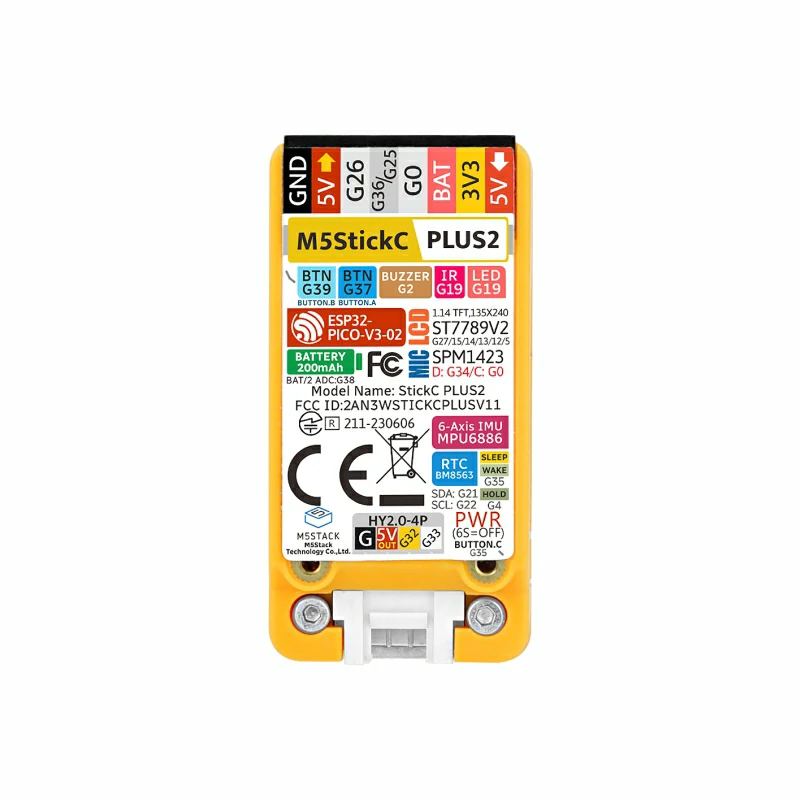
\includegraphics[width=0.4\textwidth]{figures/fig-m5stickc-plus2}
\caption{The M5StickC Plus2 wearable device. The ESP32-PICO-V3-02 system-on-chip,
the six-axis IMU (MPU6886), and the microphone (SPM1423) are all integrated on the
board. Image: M5Stack~\cite{m5stickcplus2}.}
\label{fig:m5stickc-plus2}
\end{figure}

Two properties of this platform shape the entire data pipeline. The first is that
the device is worn on the body, which rules out a high-bandwidth tethered
connection and makes wireless streaming the practical way to obtain data from
several body locations simultaneously. The second is the limited on-chip memory:
the manufacturer datasheet gives 8\,MB of flash, 2\,MB of in-package PSRAM, and
520\,KB of on-chip SRAM. This budget is comfortable for buffering and forwarding sensor samples during
acquisition, but it is the binding constraint on the eventual on-device inference
stage treated in Section~\ref{sec:deployment}. The dataset was therefore
designed so that the same device that records the training data can, in
principle, run the trained model: the inertial and acoustic sampling rates, the
window length, and the feature representations described later in this chapter
were all chosen with that target in mind rather than for offline convenience.

During data collection both the microphone and the IMU were used. The microphone
is single-channel, so each device produced one monophonic audio stream alongside
its six-axis inertial stream.

\section{Assembly Scenario and Activity Taxonomy}
\label{sec:taxonomy}

Recordings were carried out in the Future Work Lab at Fraunhofer IPA in Stuttgart,
a laboratory configured for research on human--machine interaction in
manufacturing {[}CITATION{]}.
The environment provides a workbench with parts, hand tools, and fasteners, so
that a manual assembly task can be performed under controlled but realistic
conditions.

Data were recorded from two participants over three sessions. In each session one
participant wore the sensors and performed the task while the other operated a
handheld mobile-phone camera, following the acting participant on foot during the
segments that involved walking; the two participants exchanged roles for later
sessions. Each session consisted of a repeated assembly sequence: three
repetitions in two of the sessions and four repetitions, plus one sequence marked
invalid, in the third. Session lengths, measured from the recorded streams, were
approximately 6.7, 7.6, and 16.9 minutes, for a total of about 31 minutes of
recording (Section~\ref{sec:protocol}).

Each repetition followed the same 32-step protocol, transcribed in the annotation
records. The participant begins at the bench, walks to a supply table, and
carries parts back; stacks three parts so that they align; seats them with a
hammer; measures the assembly with a scale; passes four screws through the
aligned parts by hand; drives the screws with a powered screwdriver; and places
the finished item in a storage compartment beside the bench. The remainder of
each repetition reverses the process, loosening and removing the screws and
returning the parts to their boxes. Because the same operations recur several
times per repetition, the screwdriving class dominates the dataset
(Section~\ref{sec:stats}).

Video of each session was annotated with a larger set of labels than the dataset
finally uses. Across sessions the coded label set contained fifteen to eighteen
activity labels, including narration (\texttt{speech}), the disassembly actions
(\texttt{screw\_loosening}, \texttt{remove\_screws}, \texttt{store\_part}), a rare
\texttt{pick\_container} action, and in one session the postures \texttt{sit} and
\texttt{stand}. The modelling taxonomy retains the ten classes listed in
Table~\ref{tab:activity-classes}, which cover the assembly half of the task
together with locomotion and rest. \texttt{screw\_loosening} was merged into
\texttt{screw\_tightening}: the two actions use the same powered screwdriver and
differ only in rotation direction, producing near-identical inertial and acoustic
signatures that a two-second window cannot reliably separate. This merge accounts
for the class's size: the 518 \texttt{screw\_tightening} windows in
Table~\ref{tab:activity-classes} include both tightening and loosening instances.
The remaining labels (\texttt{speech}, \texttt{remove\_screws},
\texttt{store\_part}, \texttt{pick\_container}, and, in one session,
\texttt{sit}/\texttt{stand}) were excluded rather than merged. The class
descriptions in Table~\ref{tab:activity-classes} are operational summaries taken
from the 32-step protocol; the typical instance duration is the mean length of a
coded activity segment, averaged over the three sessions.

\begin{table}[htbp]
\centering
\small
\setlength{\tabcolsep}{3.5pt}
\renewcommand{\arraystretch}{1.15}
\begin{tabularx}{\textwidth}{|p{2.4cm}|X|c|r|}
\hline
\textbf{Class} & \textbf{Operational description (from the recording protocol)}
 & \textbf{Typ.\ dur.} & \textbf{Win.} \\
\hline
\texttt{idle} & Standing at the bench without performing a task. & 4--12\,s & 45 \\
\texttt{walk} & Walking between the workstation and the supply table. & $\approx$5\,s & 73 \\
\texttt{carry\_\allowbreak container} & Carrying the parts container between the supply table and the workstation. & 5--9\,s & 56 \\
\texttt{place\_\allowbreak container} & Setting the parts container down on the work surface. & 3--5\,s & 35 \\
\texttt{assemble\_\allowbreak parts} & Stacking three parts on the workstation so that they align and fit together. & 10--19\,s & 143 \\
\texttt{hammering} & Striking the stacked parts with a hammer to seat them. & 6--11\,s & 85 \\
\texttt{measuring} & Measuring the length and width of the assembled part with a scale. & 8--9\,s & 93 \\
\texttt{insert\_\allowbreak screws} & Passing four screws through the aligned parts by hand. & 19--22\,s & 219 \\
\texttt{screw\_\allowbreak tightening} & Driving screws with a powered screwdriver; includes loosening actions merged into this class (Section~\ref{sec:taxonomy}). & 22--31\,s & 518 \\
\texttt{compartment\_\allowbreak interaction} & Opening and closing the storage compartment beside the bench. & 5--11\,s & 113 \\
\hline
\multicolumn{3}{|l|}{\textbf{Total paired windows}} & \textbf{1380} \\
\hline
\end{tabularx}
\caption{Activity classes in the modelling dataset. Descriptions are taken from
the 32-step assembly protocol. ``Typ.\ dur.'' is the range of mean coded-segment
durations across the three recording sessions; for \texttt{screw\_tightening} it
covers both the tightening and the merged loosening segments. ``Win.'' is the
number of two-second windows per class in the final dominant-wrist dataset
(Section~\ref{sec:stats}).}
\label{tab:activity-classes}
\end{table}

\section{Data-Collection Firmware}
\label{sec:firmware}

The same custom firmware was installed on all of the devices, written in C++ and
based on the Arduino framework. Its only task during acquisition is to sample the
two sensors and forward every sample to a host computer with enough timing
information for the streams to be reassembled and aligned afterwards. It performs
no filtering, no feature extraction, and no on-device storage. This section
explains the data acquisition architecture and the decisions behind it, rather
than the source code.

\subsection{Dual-Stream UDP Architecture}
\label{sec:udp}

The inertial and acoustic data are transmitted as two separate streams over
Wi-Fi using the User Datagram Protocol (UDP). One port receives inertial packets
and another receives audio packets, so that a receiver does not need to inspect
packet contents to separate the two modalities. UDP was preferred to a
connection-oriented protocol since it introduces no retransmission or reordering
delay, keeping the sender simple and the timing of transmitted packets close to
the timing of the underlying samples; the trade-off is that lost packets are not
retransmitted by the transport and must be detected and handled in post-processing
{[}CITATION{]}.

Each time a new IMU sample becomes available, an inertial packet is created that
contains the six inertial values as text, a sequence number, and a device
timestamp. Each audio packet has a sequence number, a sample count, a device
timestamp, and a fixed-size block of pulse-code-modulated (PCM) samples. Since
multiple devices send to the same host on the same two ports, the receiver logs
the source address of each packet it receives and uses it to differentiate the
streams by device. Figure~\ref{fig:acq-architecture} shows the end-to-end
acquisition path.

\begin{figure}[!ht]
\centering
\makebox[\textwidth][c]{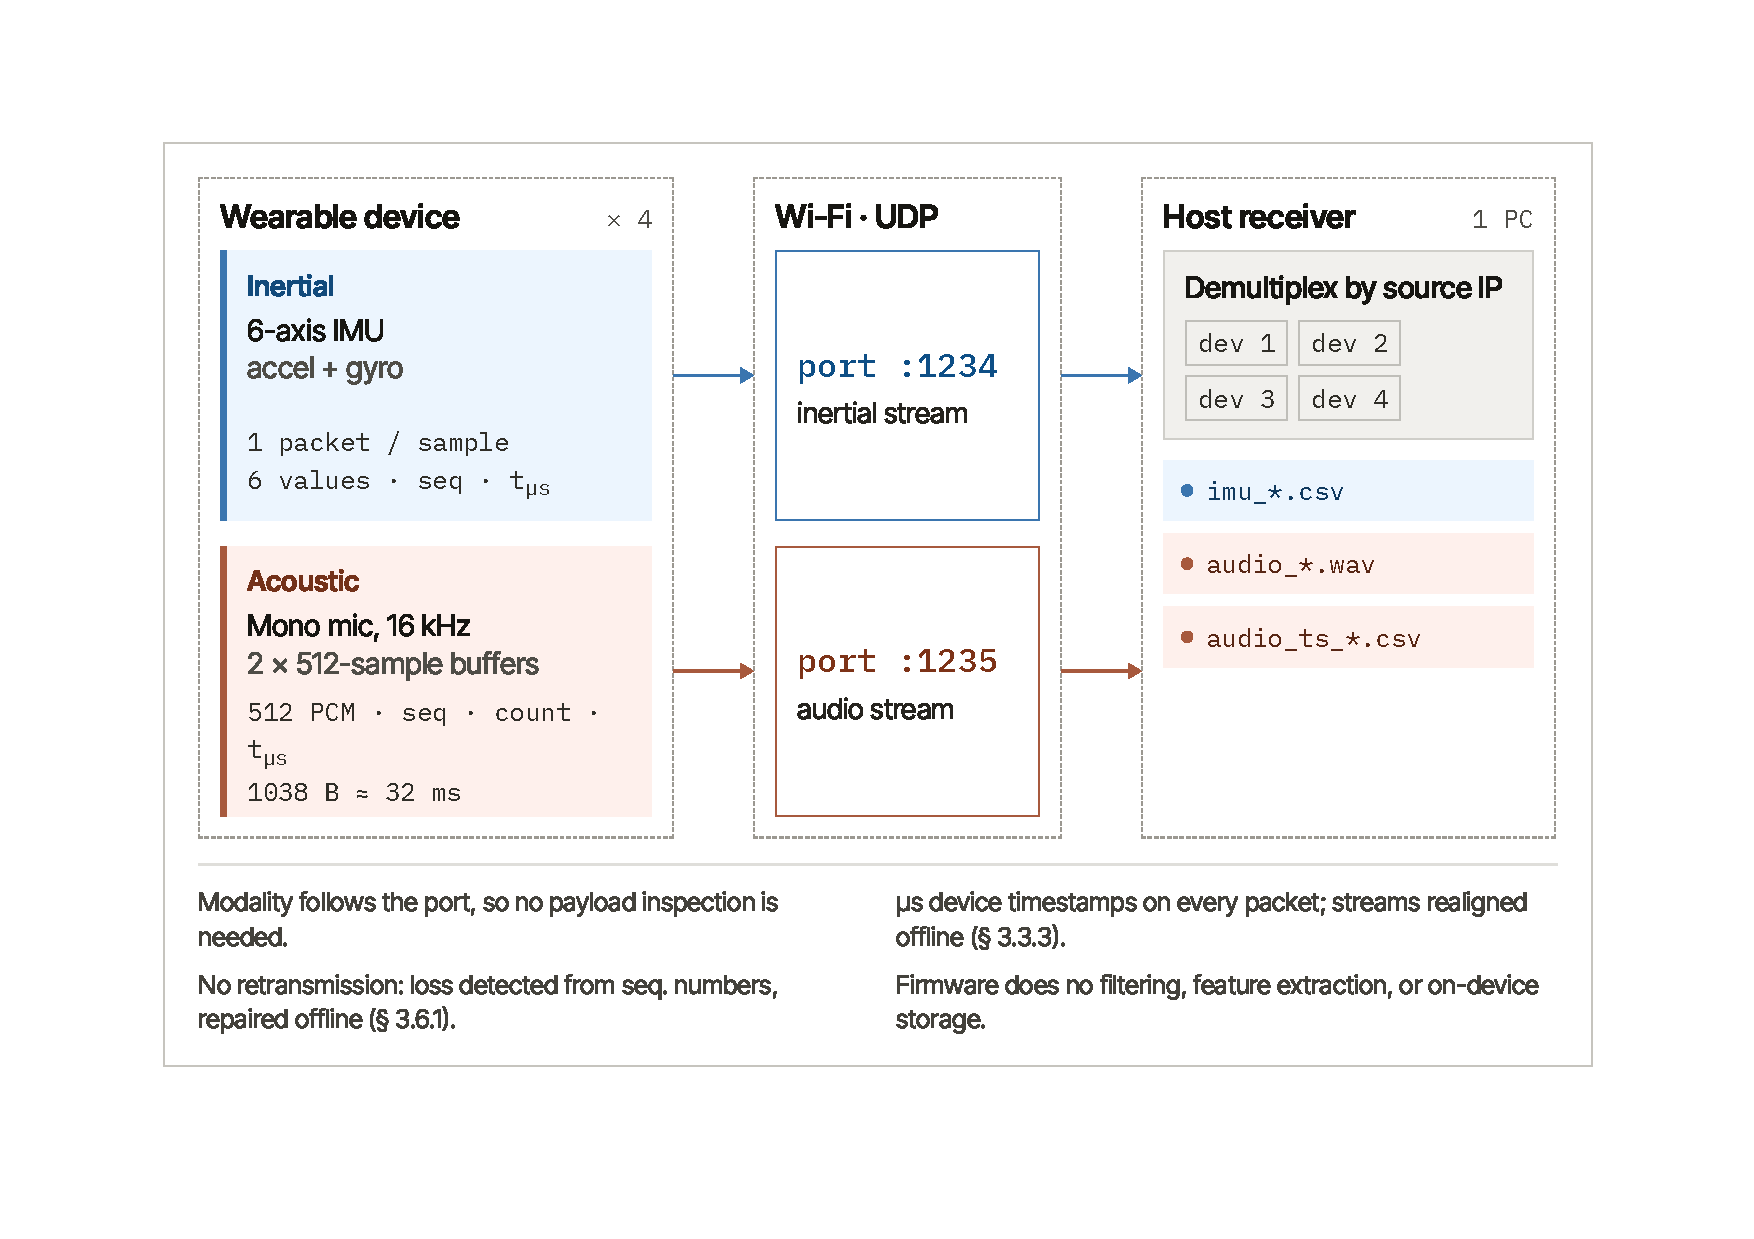
\includegraphics[width=1.1\textwidth]{figures/fig-acq-architecture}}
\caption{Architecture of the multimodal data-acquisition system. Each of the four
wearable devices samples an IMU and a microphone independently, timestamps and
frames the samples, and streams them as two separate UDP streams (inertial on one
port, audio on another) to a single host, which separates the devices by packet
source address and writes raw per-device files.}
\label{fig:acq-architecture}
\end{figure}

\subsection{Audio Double-Buffering and Packet Framing}
\label{sec:buffering}

Audio is captured continuously, so the firmware cannot stall the microphone
driver while a packet is being transmitted. To avoid this, two 512-sample buffers
are used alternately: while the driver fills one buffer, the previously filled
buffer is transmitted, and once a buffer is full, the roles swap. This prevents
new samples from overwriting data that has not yet been transmitted and keeps the
capture cadence regular.

The buffer size also determines the size of each audio packet. A 512-sample
block at a 16\,kHz sampling rate corresponds to 32\,ms of audio. Together with a
header carrying the sequence number, sample count, and timestamp, this produces a
packet of 1038\,bytes, which is well below the 1500-byte Ethernet MTU (Maximum
Transmission Unit), so every audio packet can be transmitted as a single,
unfragmented UDP datagram. Keeping packets under the MTU matters because IP
fragmentation of a UDP datagram means that losing any one fragment discards the
whole datagram, which can increase the effective audio packet loss rate
{[}CITATION{]}.

\subsection{Microsecond Timestamping and Sequence Numbering}
\label{sec:timestamps}

Each packet, inertial and acoustic, carries a timestamp taken from the device's
microsecond counter at the moment the packet is assembled, together with a
monotonically increasing sequence number. These two fields serve different
purposes. The sequence number makes packet loss detectable: a gap between
consecutive received sequence numbers means a lost packet, independent of any
timing assumption. The timestamp makes the true timing of a recording session
recoverable: it allows the elapsed time between the first and last samples to be
determined, which is later used for clock-drift correction in
Section~\ref{sec:conditioning}. It also provides the temporal reference needed to
align the inertial and acoustic streams from the same device.

The microsecond resolution is more than sufficient for this purpose: it is far
finer than the interval between individual inertial samples and than the interval
between consecutive audio packets, so timestamp quantisation does not introduce a
meaningful limitation to the alignment accuracy. The devices' timestamps cannot be
compared directly with one another, however, since the individual devices do not
share a common clock. The video reference described in
Section~\ref{sec:annotation} is therefore used to synchronise the various
devices.

\subsection{Multi-Device Capture and Body Placements}
\label{sec:placements}

In each recording session, four sensor devices were worn: one on the dominant
wrist, one on the non-dominant wrist, one at the waist, and one on the leg. All
four devices simultaneously recorded inertial and acoustic data and streamed
them to the host system. Recording at several body locations was a deliberate
design choice: it made it possible to capture potentially useful information
from different parts of the body and offered redundancy against a device failing
during a recording session.

However, not all of the recorded data were used to train the model.
Table~\ref{tab:placements} summarises the sensor data recorded and the data
finally input to the modelling pipeline. The models presented in this thesis use
only the dominant-wrist inertial data and the dominant-wrist microphone data.

During preprocessing, windows were first created for all four sensor locations
and placed in their respective session directories. These windows used the same
naming convention across all placements, based on the activity, window start
time, and window index on the shared video-aligned timeline. This naming
convention persisted when the windows were subsequently consolidated into one
directory, so each window was retained as a single file. A byte-level comparison
of the retained inertial and audio files indicated that they are those of the
dominant-wrist device. Non-dominant-wrist, waist, and leg data are thus available
in the original session data, but not in the modelling dataset.

The data from the leg-worn sensor package were excluded after inspection of the
recorded signals. The leg inertial data contained relatively little
activity-specific information for the bench-based assembly tasks, apart from
activities such as walking. Likewise, the leg microphone primarily recorded
ambient noise and captured the assembly activities poorly. This thesis also did
not use the inertial data of the non-dominant wrist and waist as model inputs.
Integrating information across more than one body location, at the feature level
or at the decision level, is instead noted as a direction for future work,
addressed in Chapter~\ref{ch:conclusion}.

\begin{table}[htbp]
\centering
\renewcommand{\arraystretch}{1.2}
\begin{tabularx}{\textwidth}{|l|C|C|C|}
\hline
\textbf{Placement} & \textbf{Modalities recorded}
 & \textbf{IMU as model input} & \textbf{Audio as model input} \\
\hline
Dominant wrist     & inertial + audio & yes & yes \\
Non-dominant wrist & inertial + audio & no  & no  \\
Waist              & inertial + audio & no  & no  \\
Leg                & inertial + audio & no  & no  \\
\hline
\end{tabularx}
\caption{Body placements: data recorded during acquisition versus data used as
model input in the final pipeline. Only the dominant-wrist inertial and acoustic
streams reach the model.}
\label{tab:placements}
\end{table}

\section{Recording Protocol}
\label{sec:protocol}

The same procedure was followed for each recording session. All four devices
were worn by the acting participant and fastened with straps to keep the sensor
axes fixed relative to the body segment to which they belonged. Before recording
started, all devices were checked to ensure that they were connected and
transmitting data correctly. The participant then repeated the set of predefined
assembly steps at the workbench while the second participant filmed the assembly
sequence with a handheld phone. The host computer displayed the incoming packets
from all four devices, so that a disconnection or a sustained loss of packets
could be noticed; no session required a restart.

Table~\ref{tab:sessions} provides an overview of the recorded sessions. The
session durations were calculated from the recorded inertial streams, and the
number of two-second windows was counted from the final dataset. The three
sessions contributed 352, 371, and 657 windows. This class imbalance, as
discussed in Section~\ref{sec:stats}, is mostly due to the recording protocol:
some actions, such as screwdriving, were performed several times within each
repetition, whereas other actions, such as placing a container, occurred only
once per repetition.

\begin{table}[htbp]
\centering
\small
\setlength{\tabcolsep}{4pt}
\renewcommand{\arraystretch}{1.2}
\begin{tabular}{|c|p{3.9cm}|c|c|c|}
\hline
\textbf{Part.} & \textbf{Session (project label)} & \textbf{Duration}
 & \textbf{Reps} & \textbf{Windows} \\
\hline
P2 & First session, all four placements & $\approx$6.7\,min & 3 & 352 \\
P1 & Three repetitions                  & $\approx$7.6\,min & 3 & 371 \\
P2 & Four repetitions, one invalid      & $\approx$16.9\,min & 4\,$(+1)$ & 657 \\
\hline
\multicolumn{2}{|l|}{\textbf{Total}} & \textbf{$\approx$31.2\,min} & & \textbf{1380} \\
\hline
\end{tabular}
\caption{Data-acquisition sessions. ``Session'' paraphrases the folder label used
in the project records. ``$(+1)$'' denotes one further sequence marked invalid and
set aside.}
\label{tab:sessions}
\end{table}

\section{Ground-Truth Annotation from Synchronised Video}
\label{sec:annotation}

The sensor recordings provide motion and acoustic information but do not contain
activity labels. The ground truth was therefore obtained from the recorded
video, which provides a visual reference for determining which activity was
being performed at a given point in time. The annotated video intervals were
then transferred to the sensor recordings. This process requires the video and
sensor data to be placed on a common timeline and the activities to be
represented as defined time intervals.

\subsection{Determination of the Audio-Video Offset}
\label{sec:offset}

The video and sensor recordings were started independently, meaning that their
time origins were not identical. Before the video annotations could be mapped
to the sensor data, a temporal offset between the two recordings had to be
determined.

The offset was calculated by finding an event that is clearly identifiable in
both the video and the recorded audio. The audio from the sensor side was
analysed in Audacity~\cite{audacity} to find the corresponding transient, which
was located within a millisecond. The same event, a spoken cue that the
participant announced at the start and end of each assembly sequence, was then
found in the video's audio track. The difference between the event times in the
sensor recording and the video provides the required temporal offset.

For instance, the offset measured for one session is 3.857\,seconds. This value
is used for the synchronisation procedure to take out the same amount of data
from the beginning of each sensor stream, so that the beginning of the sensor
timeline becomes the zero point of the video. In each recording session, the
offset was determined independently and applied to the synchronised streams used
in this thesis. This step appears in the full preprocessing pipeline shown in
Figure~\ref{fig:pipeline}.

\subsection{Interval Labels and Sample-Level Label Embedding}
\label{sec:labels}

The activities were annotated directly from the video using
BORIS~\cite{friard2016boris}, a tool for behavioural observation and event
logging. Every annotation specifies a start time, an end time, and an activity
label on the video timeline. The annotations were exported to a table with the
columns \texttt{Label}, \texttt{Start}, and \texttt{End}.

These annotation intervals were then moved to the sensor data. For each
inertial sample, its timestamp relative to the beginning of the recording was
compared with the annotated intervals. If the timestamp was within an activity
interval, the associated activity label was attributed to the sample. Samples
that were not part of any of the annotated intervals were assigned a reserved
\texttt{unlabeled} marker. This avoids assigning an activity label to
transition periods or moments in which no specific task was being performed.

The assigned label was saved as a separate column along with the inertial
measurements, and thus the inertial recording was transformed into a labelled
time series. The audio stream was labelled using the same temporal reference.
Since the audio and inertial data originate from the same device and were
aligned to the video timeline, an audio segment corresponds to the activity
represented by the inertial samples covering the same time interval.
Consequently, transitions and untasked periods remain explicitly represented as
\texttt{unlabeled}. Their treatment during the subsequent windowing process is
described in Section~\ref{sec:windowing}.

\section{Signal Conditioning}
\label{sec:conditioning}

Before the data were divided into windows, the recorded streams were processed
to compensate for transmission-related artefacts and differences in the device
clocks. Next, the inertial and acoustic data were brought to fixed sampling
rates to ensure consistent processing across all the recordings.

The conditioning process was repeated for each of the devices and yielded
continuous, uniformly sampled, and temporally aligned inertial and acoustic
streams. The entire pre-processing chain is shown in Figure~\ref{fig:pipeline}.

\begin{figure}[htbp]
\centering
\begin{tikzpicture}[node distance=3.5mm, every node/.style={blk, text width=6.6cm}]
  \node (raw) {Per-device raw streams (\texttt{imu}, \texttt{audio}, \texttt{audio\_ts})};
  \node (drop) [below=of raw] {Audio-dropout detection; silent (zero) padding of missing chunks};
  \node (drift) [below=of drop] {Clock-drift correction: sample rate re-estimated from first/last timestamp};
  \node (trim) [below=of drift] {Inertial head-trim to the audio start time};
  \node (vid) [below=of trim] {Video-offset trim to the annotation zero mark};
  \node (lab) [below=of vid] {Interval-label embedding (BORIS export)};
  \node (split) [below=of lab, text width=6.6cm]
        {Inertial: mean-bin decimation to 80\,Hz \quad$|$\quad Audio: resample to 16\,kHz};
  \node (seg) [below=of split] {Continuous activity-segment extraction ($\geq 2$\,s)};
  \node (win) [below=of seg] {Two-second windowing, 50\,\% overlap, majority-vote label, $\geq 70$\,\% label coverage};
  \node (out) [below=of win] {Labelled paired inertial/audio windows};
  \foreach \a/\b in {raw/drop, drop/drift, drift/trim, trim/vid, vid/lab, lab/split,
                     split/seg, seg/win, win/out}
    \draw[flow] (\a) -- (\b);
\end{tikzpicture}
\caption{Signal-conditioning and windowing pipeline, applied per device. The
inertial and acoustic branches are brought to fixed rates before both are cut on
the same window boundaries.}
\label{fig:pipeline}
\end{figure}

\subsection{Packet-Loss Detection and Audio-Dropout Reconstruction}
\label{sec:dropout}

Missing audio packets appear as gaps in the recorded waveform. Since each audio
packet contains an arrival timestamp and a fixed number of samples, the
expected time between consecutive packets can be determined. At a sampling rate
of 16\,kHz, for example, a packet containing 512 samples represents 32\,ms of
audio, so under normal conditions consecutive packets are expected to be
separated by approximately 32\,ms.

A larger time gap between two received packets indicates that one or more
packets may have been lost. The number of missing packets is estimated from the
observed time difference using
\[
\operatorname{round}\!\left(\frac{\Delta t - T_{\mathrm{packet}}}{T_{\mathrm{packet}}}\right),
\]
where $\Delta t$ denotes the observed time difference between two consecutive
received packets and $T_{\mathrm{packet}}$ denotes the expected packet
interval. For the 16\,kHz audio stream with 512 samples per packet,
$T_{\mathrm{packet}} = 32\,\mathrm{ms}$. For example, if two received packets
are separated by 96\,ms, the equation gives
\[
\operatorname{round}\!\left(\frac{96 - 32}{32}\right) = 2.
\]
This means that two packets are assumed to be missing between the two received
packets.

If a packet is detected as missing, a block of 512 zero-valued samples is
inserted at the appropriate location in the waveform. This approach does not
attempt to reconstruct the missing acoustic content. Instead, its purpose is to
preserve the correct duration and temporal position of the surrounding signal
so that subsequent time-frequency analysis is not affected by a shortened audio
stream. The missing regions are therefore represented as silence. This is a
conservative approach, as it introduces no artificial acoustic events, at the
cost of a short period of artificially silent audio.

The fraction of reconstructed audio, computed from the raw per-device
packet-arrival timestamps, is 0.15--0.40\,\% per session and about 0.33\,\%
overall for the dominant wrist (Section~\ref{sec:quality}); this is numerically
identical to the packet-loss rate, since every missing packet is exactly 512
samples of silence.

The sequence numbers are used to detect the loss of packets in the inertial
streams as well. In the dominant-wrist stream, the packet-loss rates were
0.056\,\%, 0.022\,\%, and 0.031\,\% for the three sessions, respectively, and
roughly 0.035\,\% overall (Section~\ref{sec:quality}). As described in
Section~\ref{sec:decimation}, the short gaps in the inertial data were then
filled by linear interpolation on the resampled time grid.

\subsection{IMU Decimation to 80\,Hz}
\label{sec:decimation}

The inertial stream is delivered at the device native rate, measured at
249.6--249.9\,Hz across the three sessions from the devices' microsecond
timestamps. This is consistent with the recovered design notes but not with the
firmware's own in-code comment, which labels the relevant configuration call
``100\,Hz''; the discrepancy has no effect on the modelling data, since
decimation always targets a fixed 80\,Hz regardless of the input rate. The
stream is reduced to this uniform 80\,Hz for modelling.

The reduction is performed by mean binning. The stream is divided into
consecutive 12.5\,ms bins, matching the desired sampling period at 80\,Hz, and
the inertial values in each bin are averaged to produce one output sample. If a
bin contains no samples, for instance because of packet loss, its value is
estimated by linear interpolation between the surrounding samples. The label
column is decimated separately by taking the most frequent label in each bin.
The resulting stream sits on an exact 80\,Hz grid, which removes the small
timing irregularities of the native stream.

Mean binning also provides a simple form of smoothing, although it is not used
as a substitute for a specifically designed anti-aliasing filter. In
particular, averaging within each bin attenuates signal components above the
new Nyquist frequency of 40\,Hz to some degree, but no filter with a defined
passband or stopband was designed as part of this preprocessing step.

The rate of 80\,Hz was selected based on the target platform and the
anticipated nature of the activities to be captured. The sampling rate is
intended to retain the frequency content relevant to the wrist movements
involved in manual assembly, while substantially reducing the amount of
inertial data and the resulting model input size {[}CITATION{]}. This
reduces the inertial sampling rate by roughly a factor of three compared with
the measured native rate.

\subsection{Audio Resampling to a Strict 16\,kHz Timeline}
\label{sec:resample}

Following clock-drift correction, every audio stream is resampled from its
effective sampling rate to a strict 16\,kHz timeline using the band-limited
resampler in librosa~\cite{mcfee2015librosa}. The resulting signal is stored as
16-bit PCM.

Using a fixed sampling rate ensures that the number of audio samples directly
corresponds to a fixed duration. This is crucial for the windowing and
feature-extraction stages that follow, because each example must span the same
time interval and generate a consistent input representation. The sampling
rate of 16\,kHz is also sufficient to capture the frequency range considered
relevant for the recorded assembly activities, which include impulsive and
periodic sounds such as those generated when hammering and screwdriving. It is
also consistent with the sampling rate used by the audio feature-extraction
pipeline described in Chapter~\ref{ch:method}.

\section{Window Generation and Labelling}
\label{sec:windowing}

After signal conditioning, the synchronised streams are first cut into
continuous activity segments. Each segment is associated with one annotated
activity interval and is only considered for further processing if it has a
duration of at least two seconds. These segments are later split into
equal-size windows for classification.

Each window has a duration of two seconds, with a 50\,\% overlap between
consecutive windows, so a new window starts every one second. Overlapping
windows are common in activity recognition because they increase the number of
training examples and reduce the chance that a short activity is sliced at a
window boundary~\cite{bulling2014tutorial}; the selected two-second window
length and 50\,\% overlap are within the range commonly used in wearable
HAR~\cite{banos2014window}. For the selected sampling rates, each two-second
window contains 160 inertial samples at 80\,Hz and 32\,000 audio samples at
16\,kHz. Both modalities are segmented using the same temporal boundaries on
the shared timeline, so each inertial window has a corresponding audio window
of the same span; the two together form one paired multimodal example.

The activity label of each window is decided using majority vote. The vote
counts only samples that carry a valid activity label; samples tagged as
\texttt{unlabeled} (Section~\ref{sec:labels}) are not included. The activity
that appears most often among the labelled samples is assigned to the window.

To prevent transition periods from becoming part of the training data, a
minimum label-coverage threshold of 70\,\% is applied. A window is kept only if
at least 70\,\% of its samples have a valid activity label. A window with a high
proportion of \texttt{unlabeled} samples is not assigned to an activity class
but is discarded instead, usually at transitions between activities. This
method keeps windows with many transitions out of the training data while
preserving windows that may have some activity-boundary overlap.
Figure~\ref{fig:windowing} shows the full window generation and labelling
process.

\begin{figure}[htbp]
\centering
\resizebox{\textwidth}{!}{%
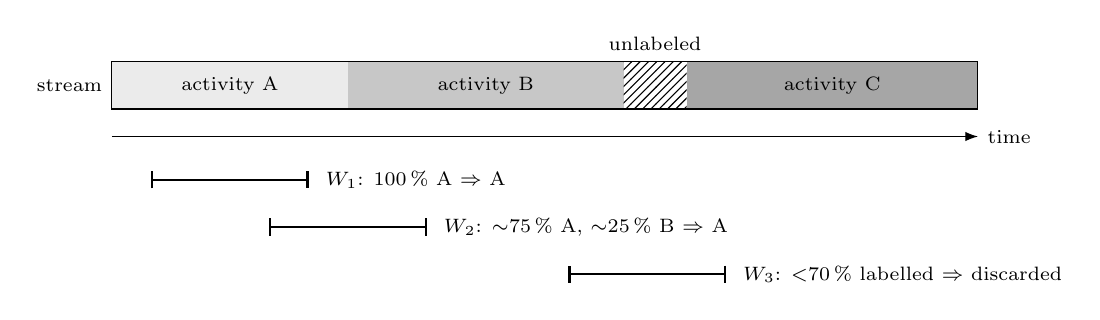
\begin{tikzpicture}[x=1cm, y=1cm, font=\scriptsize]
  % labelled stream strip: 1 cm == 1 s
  \fill[black!8]  (0,0)   rectangle (3,0.6);
  \fill[black!22] (3,0)   rectangle (6.5,0.6);
  \fill[pattern=north east lines] (6.5,0) rectangle (7.3,0.6); % unlabeled
  \fill[black!35] (7.3,0) rectangle (11,0.6);
  \draw (0,0) rectangle (11,0.6);
  \node at (1.5,0.3)  {activity A};
  \node at (4.75,0.3) {activity B};
  \node at (9.15,0.3) {activity C};
  \node[above] at (6.9,0.62) {unlabeled};
  \node[left] at (0,0.3) {stream};
  \draw[-{Latex[length=1.6mm]}] (0,-0.35) -- (11,-0.35) node[right] {time};
  % stacked 2 s windows (2 cm wide), each with its label to the right
  \foreach \y/\xa/\txt in {%
      -0.9/0.5/{$W_1$: 100\,\% A $\Rightarrow$ A},
      -1.5/2.0/{$W_2$: $\sim$75\,\% A, $\sim$25\,\% B $\Rightarrow$ A},
      -2.1/5.8/{$W_3$: $<$70\,\% labelled $\Rightarrow$ discarded}}{
    \pgfmathsetmacro{\xb}{\xa+2}
    \draw[|-|, thick] (\xa,\y) -- (\xb,\y);
    \node[right] at (\xb,\y) {\ \txt};
  }
\end{tikzpicture}}
\caption{Window generation and majority-vote labelling. Two-second windows advance
in one-second steps ($W_1$, $W_2$, $W_3$ shown stacked for clarity). A window takes
the majority activity among its labelled samples; a window whose labelled coverage
falls below 70\,\%, such as one spanning the transition region, is discarded.}
\label{fig:windowing}
\end{figure}

Windowing was carried out for all four body placements, producing one set of
labelled inertial and audio windows per placement, organised by class. The
per-placement sets that are not used for modelling contain fifteen activity labels
each.

\section{Dataset Statistics, Class Distribution, and Imbalance}
\label{sec:stats}

The dataset used for modelling is the dominant-wrist subset. It has 1380 paired
inertial and audio windows for the ten activity classes outlined in
Table~\ref{tab:activity-classes}. The data come from two participants and
three recording sessions and represent roughly 23 minutes of windowed activity
out of the 31 minutes of recorded data; the remaining time is not part of the
modelling dataset because of excluded classes, the invalid sequence, and
windows removed around activity transitions.

Each inertial window contains a $160 \times 6$ array of accelerometer and
gyroscope measurements sampled at 80\,Hz. Each corresponding audio window
contains 32\,000 mono samples at 16\,kHz. Table~\ref{tab:composition}
summarises the composition of the dataset, and Figure~\ref{fig:classdist}
shows the distribution of windows across the activity classes.

\begin{table}[htbp]
\centering
\begin{tabular}{|l|l|}
\hline
\textbf{Property} & \textbf{Value} \\
\hline
Paired inertial/audio windows & 1380 \\
Activity classes              & 10 \\
Participants                  & 2 \\
Recording sessions            & 3 \\
Windowed activity             & $\approx$23\,min \\
Window length                 & 2\,s \\
Window stride                 & 1\,s (50\,\% overlap) \\
Minimum label coverage        & 70\,\% \\
Inertial window               & $160 \times 6$ at 80\,Hz \\
Audio window                  & 32\,000 samples, mono, 16\,kHz \\
Inertial channels             & acc\_x, acc\_y, acc\_z, gyro\_x, gyro\_y, gyro\_z \\
\hline
\end{tabular}
\caption{Composition of the dominant-wrist modelling dataset.}
\label{tab:composition}
\end{table}

\begin{figure}[htbp]
\centering
\resizebox{\textwidth}{!}{%
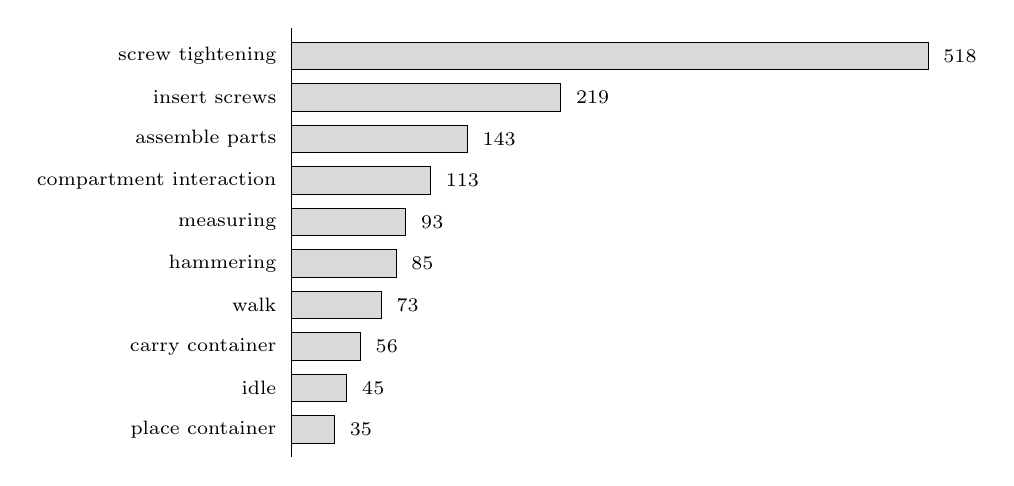
\begin{tikzpicture}[x=1pt, y=1pt]
  \foreach [count=\i] \name/\val in {%
      screw tightening/518, insert screws/219, assemble parts/143,
      compartment interaction/113, measuring/93, hammering/85, walk/73,
      carry container/56, idle/45, place container/35}{
    \pgfmathsetmacro{\w}{\val/518*230}
    \pgfmathsetmacro{\yb}{-\i*15}
    \pgfmathsetmacro{\yt}{\yb+10}
    \pgfmathsetmacro{\ym}{\yb+5}
    \pgfmathsetmacro{\wl}{\w+2}
    \fill[black!15] (0,\yb) rectangle (\w,\yt);
    \draw (0,\yb) rectangle (\w,\yt);
    \node[left,  font=\scriptsize] at (-2,\ym) {\name};
    \node[right, font=\scriptsize] at (\wl,\ym) {\val};
  }
  \draw (0,0) -- (0,-155);
\end{tikzpicture}}
\caption{Number of two-second windows per activity class in the dominant-wrist
dataset ($n = 1380$). The distribution is dominated by the screwdriving classes;
\texttt{screw\_tightening} alone accounts for about 38\,\% of the windows and the
two screwdriving classes together for more than half.}
\label{fig:classdist}
\end{figure}

There is a significant imbalance in the class distribution. The smallest
class, \texttt{place\_container}, contains only 35 windows, roughly one
fifteenth of the largest. This imbalance is primarily due to the design of the
task: actions such as screwdriving were repeated numerous times during each
session, while other activities such as moving a container or walking were
repeated only a few times. Consequently, the imbalance persists in the dataset
and is not corrected during preprocessing. How it is handled in training and
evaluation is detailed in Chapter~\ref{ch:method}, and its impact on the
findings in Chapter~\ref{ch:discussion}.

The number of windows discarded during windowing because they failed the
70\,\% label-coverage requirement was not recorded.

\section{Data-Quality Assessment and Known Artefacts}
\label{sec:quality}

There are a number of characteristics of the data that are important to
consider. These characteristics do not prevent the dataset from being used for
the experiments in this thesis, but they define the limits of what can
reasonably be concluded from those experiments. Table~\ref{tab:quality}
summarises the primary data-quality indicators that could be established.

\begin{table}[htbp]
\centering
\footnotesize
\setlength{\tabcolsep}{3.5pt}
\renewcommand{\arraystretch}{1.2}
\begin{tabularx}{\textwidth}{|p{3.5cm}|p{2.3cm}|X|}
\hline
\textbf{Indicator} & \textbf{Value} & \textbf{Notes} \\
\hline
Inertial packet loss (dominant wrist) & 0.022--0.056\,\% per session &
  From sequence-number gaps; $\approx$0.035\,\% overall. Below the 1\,\% design
  target. \\
Audio packet loss (dominant wrist) & 0.15--0.40\,\% per session; $\approx$0.33\,\% overall &
  From \texttt{audio\_ts} packet-arrival timestamp gaps, computed from the raw
  per-device logs. Reconstructed audio (inserted silence) is the same
  fraction, since every missing packet is exactly 512 samples. \\
Synchronisation basis & one manual event per session &
  Residual reading error and slow clock drift over a session are not
  characterised. \\
Camera & handheld, moving &
  Framing varied, but no hand action was occluded during annotation. \\
Discarded low-coverage windows & not recorded & See Section~\ref{sec:stats}. \\
\hline
\end{tabularx}
\caption{Data-quality indicators for the dataset.}
\label{tab:quality}
\end{table}

\textbf{Packet loss and audio reconstruction.} Wireless UDP transmission loses
packets. Inertial loss on the dominant-wrist stream is measured at about
0.035\,\% overall (Section~\ref{sec:dropout}). Audio loss, computed from the raw
per-device packet-arrival timestamps, is higher: 0.15--0.40\,\% per session and
about 0.33\,\% overall for the dominant wrist, roughly an order of magnitude
above the inertial loss rate. Because every missing audio packet is
reconstructed as exactly 512 samples of silence (Section~\ref{sec:dropout}), the
reconstructed-audio fraction is numerically the same figure.

\textbf{Synchronisation uncertainty.} The alignment of the sensor recordings
with the activity annotations is based on a manually identified synchronisation
event for each session, followed by a fixed offset applied to the entire
session (as described in Section~\ref{sec:offset}). There is no quantification
of the residual error caused by manual event locating, and no characterisation
of the gradual clock drift between the recordings. Majority voting applied over
two-second windows and the 70\,\% threshold for label coverage minimise the
risk of a small window alignment error affecting the label assigned to a
particular window. However, this kind of error can still change the effective
boundaries of an activity.

\textbf{Scope of the dataset.} The dataset was collected from two participants
performing a scripted assembly task in a single laboratory environment. The
final modelling data represent approximately 23 minutes of windowed activity,
with one class accounting for more than one third of all windows. The dataset
is suitable for the comparative analysis of multimodal fusion methods and
on-device feasibility undertaken in this thesis. Its size and limited variation
do not make it suitable for assessing how the resulting models would perform
for different participants, assembly tasks, or environments. These limitations
are addressed in more detail in Chapter~\ref{ch:discussion}, which also
discusses their effect on the experimental results.

\section{Chapter Summary}
\label{sec:ch3-summary}

This chapter described the construction of the multimodal dataset. Inertial and
acoustic data were streamed over Wi-Fi from four M5StickC Plus2 devices worn at the
wrists, waist, and leg, using a UDP-based firmware that timestamps and
sequence-numbers every packet so that the streams can be realigned after
transmission. Two participants performed a scripted manual assembly task across
three sessions in the Fraunhofer IPA Future Work Lab, alternating between
performing the task and filming it on a handheld phone. Activity intervals were
coded from the video in BORIS and transferred onto the sensor timeline after the
sensor-to-video offset was fixed from a shared event located in Audacity. Each
device stream was then corrected for audio dropouts and clock drift, decimated to
80\,Hz for the inertial channels and resampled to 16\,kHz for audio, and segmented
into overlapping two-second windows labelled by majority vote subject to a 70\,\%
coverage threshold. The modelling dataset used in the remainder of this thesis is
the dominant-wrist subset: 1380 paired inertial and audio windows over ten activity
classes, single-channel audio, with a strong class imbalance dominated by
screwdriving actions and with the data-quality limitations set out in
Section~\ref{sec:quality}. This dataset is the common input to all of the models
and experiments described in the following chapters.
 % Load Data from File chapter3.tex

\chapter{Model Design, Training and Deployment}
% Chapter 4 -- Model Design and Training
% Figures are authored in TikZ so the chapter compiles without external assets.
% Placeholders [CITATION: ...] mark references still to be added.

\label{ch:method}

\tikzset{
  blk/.style={draw, rounded corners=2pt, align=center, inner sep=4pt,
              minimum height=8mm, font=\footnotesize},
  grp/.style={draw, dashed, rounded corners=3pt, inner sep=6pt},
  flow/.style={-{Latex[length=2mm]}, thick},
}

This chapter describes the models used for activity recognition and the
procedure used to train and evaluate them. It begins with an overview of the
experimental design and its relation to the research questions. It then covers
the input representations derived from the inertial and acoustic windows of
Chapter~\ref{ch:data}, the single-modality models, the three fusion strategies,
and a classical baseline using hand-crafted features. It closes with the training
procedure and the evaluation protocol that all models share. The results obtained
with these models are presented in Chapter~\ref{ch:results}, and the conversion
of selected models for execution on the wearable device is covered in
Chapter~\ref{ch:implementation}.

\section{Overview of the Experimental Design}
\label{sec:design}

The experiments compare models that differ in one respect at a time while
sharing everything else: the same windows, the same train/validation split, the
same input normalisation and the same training settings. This makes differences
in accuracy attributable to the model design rather than to differences in the
data or in the training procedure.

The models fall into four groups, each linked to one or more of the research
questions formulated in Chapter~1:

\begin{itemize}
  \item \textbf{Single-modality models} use either inertial or acoustic data
  alone. They form the reference point against which the benefit of adding audio
  is measured (RQ1, RQ3).
  \item \textbf{Fusion models} combine both modalities at different stages of
  processing: at the input level (early fusion), at the level of learned
  representations (embedding-level fusion), or at the level of class predictions
  (decision-level fusion). Their comparison addresses RQ2.
  \item \textbf{A classical baseline} based on statistical features and a random
  forest shows how much the learned models gain over a conventional approach
  (RQ3).
  \item \textbf{Reduced model variants} with fewer parameters were designed with
  the memory and computational limits of the target device in mind. They connect
  the offline comparison to the deployment study in
  Chapter~\ref{ch:implementation} (RQ4).
\end{itemize}

\begin{table}[htbp]
\centering
\small
\renewcommand{\arraystretch}{1.2}
\begin{tabularx}{\textwidth}{|p{3.1cm}|X|p{2.4cm}|p{2.6cm}|}
\hline
\textbf{Group} & \textbf{Model} & \textbf{Inputs} & \textbf{Fusion stage} \\
\hline
Single modality & IMU CNN & inertial & -- \\
Single modality & Audio CNN (GAP, GRU and hybrid pooling) & acoustic & -- \\
Early fusion & Channel concatenation (standard and small) & inertial + acoustic & input \\
Early fusion & Unified spectrogram & inertial + acoustic & input \\
Embedding-level fusion & Frozen backbones with a trained fusion head (standard and small) & inertial + acoustic & representation \\
Decision-level fusion & Weighted average with global or per-class weights (standard and small) & inertial + acoustic & prediction \\
Classical baseline & Random forest on hand-crafted features & inertial + acoustic & feature \\
\hline
\end{tabularx}
\caption{Overview of the evaluated models.}
\label{tab:model-overview}
\end{table}

All experiments use the dominant-wrist dataset described in
Chapter~\ref{ch:data}, with 2565 paired windows across nine activity classes. The
standalone audio model is the one exception: it additionally uses audio windows
from the non-dominant wrist and the waist, as explained in
Section~\ref{sec:audio-model}.

\section{Input Representations}
\label{sec:inputs}

\subsection{Inertial Windows}
\label{sec:imu-input}

Each inertial window holds 160 samples of the six channels (three-axis
acceleration and three-axis angular velocity) recorded at 80\,Hz. Before entering
a model, the window is resampled to 200 time steps by linear interpolation along
the time axis, so that all inertial models take inputs of size $200 \times 6$.
The target length of 200 was chosen to match the time resolution of the audio
spectrogram, which has 198 frames per window (Section~\ref{sec:logmel}). This
allows both modalities to share one time axis in the early fusion model
(Section~\ref{sec:early-fusion}) without coarsening the audio representation, and
using the same length in all inertial models keeps their inputs identical across
the experiments. Missing or non-finite values, which can remain at the very edges of a recording
after decimation, are replaced by zero.

Accelerometer and gyroscope channels have different physical units and value
ranges. Each channel is therefore standardised to zero mean and unit variance.
The mean and standard deviation of each channel are computed on the training
split only and then applied unchanged to the validation data, so that no
statistics of the validation set enter the training process. The same statistics
are later embedded in the device firmware, where they are applied to the live
sensor data (Chapter~\ref{ch:implementation}).

\subsection{Audio Log-Mel Spectrograms}
\label{sec:logmel}

Raw audio windows of 32\,000 samples are too long to be used directly as input
to a small model. Each window is therefore converted into a log-mel spectrogram,
a time-frequency representation that is widely used for sound classification
{[}CITATION{]}. The conversion consists of three steps:

\begin{enumerate}
  \item a short-time Fourier transform (STFT) with frames of 25\,ms (400
  samples), a hop of 10\,ms (160 samples) and an FFT length of 512;
  \item a projection of the magnitude spectrum onto 40 mel-spaced frequency bands
  between 20\,Hz and 8\,kHz {[}CITATION{]};
  \item the natural logarithm of the band energies, with a small constant
  ($10^{-6}$) added to avoid the logarithm of zero.
\end{enumerate}

A two-second window produces a spectrogram of 198 frames $\times$ 40 mel bands.
This reduces the input size by roughly a factor of four compared with the raw
waveform, while keeping the spectral and temporal structure that distinguishes,
for example, the continuous whine of a powered screwdriver from the short,
broadband impacts of hammering. As with the inertial data, the spectrogram is
standardised per mel band using the mean and standard deviation of the training
split. Figure~\ref{fig:logmel} summarises the feature extraction, and
Table~\ref{tab:inputs} lists the resulting input representations.

\begin{figure}[htbp]
\centering
\begin{tikzpicture}[node distance=3.5mm, every node/.style={blk, text width=7.2cm}]
  \node (wav) {Audio window: 2\,s, 32\,000 samples at 16\,kHz};
  \node (stft) [below=of wav] {STFT: 25\,ms frames, 10\,ms hop, FFT length 512};
  \node (mag) [below=of stft] {Magnitude spectrum (257 frequency bins per frame)};
  \node (mel) [below=of mag] {Mel filter bank: 40 bands, 20\,Hz--8\,kHz};
  \node (log) [below=of mel] {Natural logarithm, $\log(E + 10^{-6})$};
  \node (norm) [below=of log] {Per-band standardisation (training statistics)};
  \node (out) [below=of norm] {Log-mel spectrogram: 198 frames $\times$ 40 bands};
  \foreach \a/\b in {wav/stft, stft/mag, mag/mel, mel/log, log/norm, norm/out}
    \draw[flow] (\a) -- (\b);
\end{tikzpicture}
\caption{Conversion of a two-second audio window into the log-mel spectrogram used
as input to the acoustic models.}
\label{fig:logmel}
\end{figure}

\begin{table}[htbp]
\centering
\small
\renewcommand{\arraystretch}{1.2}
\begin{tabularx}{\textwidth}{|l|p{3.1cm}|p{3.3cm}|X|}
\hline
\textbf{Modality} & \textbf{Raw window} & \textbf{Model input} & \textbf{Normalisation} \\
\hline
Inertial & $160 \times 6$ at 80\,Hz & $200 \times 6$ (linear resampling) & per channel, training statistics \\
Audio & 32\,000 samples at 16\,kHz & $198 \times 40$ log-mel & per mel band, training statistics \\
\hline
\end{tabularx}
\caption{Input representations of the two modalities.}
\label{tab:inputs}
\end{table}

\section{Single-Modality Models}
\label{sec:single}

\subsection{Inertial Model}
\label{sec:imu-model}

The inertial model is a one-dimensional convolutional neural network (1D CNN)
that convolves along the time axis of the window. 1D CNNs are a common choice for
wearable activity recognition because they learn local motion patterns directly
from the raw signal and remain small enough for embedded use {[}CITATION{]}.

The network has two convolutional blocks. The first block applies 64 filters with
a kernel size of 5, followed by batch normalisation and max pooling with a factor
of 2. The second block applies 128 filters with a kernel size of 3, followed by
batch normalisation. Global average pooling then reduces the temporal dimension
to a single feature vector. This vector passes through a dense layer with 64
units, which also serves as the embedding for embedding-level fusion
(Section~\ref{sec:embedding-fusion}), and through dropout with a rate of 0.3,
before a softmax output layer with one unit per class.

\subsection{Audio Model and Temporal Pooling Variants}
\label{sec:audio-model}

The audio model treats the log-mel spectrogram as a single-channel image and
processes it with a two-dimensional CNN {[}CITATION{]}. It has two convolutional
blocks with 32 and 64 filters of size $3 \times 3$, each followed by batch
normalisation and $2 \times 2$ max pooling. The resulting feature map has a size
of $49 \times 10 \times 64$ (time $\times$ frequency $\times$ channels).

How this feature map is reduced to a single vector determines which properties of
the sound the classifier can use. Three variants were therefore evaluated
(Figure~\ref{fig:audio-variants}):

\begin{itemize}
  \item \textbf{Global average pooling (GAP).} The feature map is averaged over
  both time and frequency {[}CITATION{]}. This is the standard approach and gives a compact model. However,
  averaging over time removes the information about how the sound develops within
  the window. Two activities with a similar average spectrum but a different
  temporal pattern, such as the regular strikes of a hammer and the steady sound
  of a screwdriver, can then become hard to separate.
  \item \textbf{Recurrent pooling (GRU).} The feature map is reshaped into a
  sequence of 49 time steps with 640 features each and passed through a
  bidirectional gated recurrent unit (GRU) with 32 units per direction
  {[}CITATION{]}. The GRU summarises the sequence while keeping its
  temporal order, so the model can use rhythm and envelope information.
  \item \textbf{Hybrid pooling.} Both summaries are computed in parallel and
  concatenated: the GAP vector, which describes the average timbre of the
  window, and the GRU output, which describes its temporal structure. The
  classifier can then rely on whichever information is useful for a given class.
\end{itemize}

In all three variants, the pooled vector passes through a dense layer with 64
units and dropout with a rate of 0.4, followed by the softmax output.

\begin{figure}[htbp]
\centering
\resizebox{\textwidth}{!}{%
\begin{tikzpicture}[node distance=3.5mm and 6mm, every node/.style={blk}]
  \node[text width=3.4cm] (in) {Input\\$198 \times 40 \times 1$};
  \node[text width=3.4cm, below=of in] (c1) {Conv2D 32, $3\times3$\\BN, MaxPool $2\times2$};
  \node[text width=3.4cm, below=of c1] (c2) {Conv2D 64, $3\times3$\\BN, MaxPool $2\times2$};
  \node[text width=3.4cm, below=of c2] (fm) {Feature map\\$49 \times 10 \times 64$};
  \foreach \a/\b in {in/c1, c1/c2, c2/fm} \draw[flow] (\a) -- (\b);

  % (a) GAP
  \node[text width=2.8cm, right=12mm of in] (ga) {(a) GAP};
  \node[text width=2.8cm, below=of ga] (gd) {Dense 64\\Dropout 0.4};
  \node[text width=2.8cm, below=of gd] (go) {Softmax (9)};
  \draw[flow] (ga) -- (gd); \draw[flow] (gd) -- (go);

  % (b) GRU
  \node[text width=2.8cm, right=of ga] (ra) {(b) Reshape $49 \times 640$};
  \node[text width=2.8cm, below=of ra] (rg) {BiGRU, 32 units};
  \node[text width=2.8cm, below=of rg] (rd) {Dense 64\\Dropout 0.4};
  \node[text width=2.8cm, below=of rd] (ro) {Softmax (9)};
  \foreach \a/\b in {ra/rg, rg/rd, rd/ro} \draw[flow] (\a) -- (\b);

  % (c) hybrid
  \node[text width=2.8cm, right=of ra] (ha) {(c) GAP $\parallel$ BiGRU};
  \node[text width=2.8cm, below=of ha] (hc) {Concatenate\\(64 + 64)};
  \node[text width=2.8cm, below=of hc] (hd) {Dense 64\\Dropout 0.4};
  \node[text width=2.8cm, below=of hd] (ho) {Softmax (9)};
  \foreach \a/\b in {ha/hc, hc/hd, hd/ho} \draw[flow] (\a) -- (\b);

  \draw[flow] (fm.east) -| ($(ga.west)+(-5mm,0)$) -- (ga.west);
  \draw[flow] (fm.east) -- ++(4mm,0) |- ($(ra.north)+(0,4mm)$) -- (ra.north);
  \draw[flow] (fm.east) -- ++(4mm,0) |- ($(ha.north)+(0,4mm)$) -- (ha.north);
\end{tikzpicture}}
\caption{Audio model with a shared convolutional stem and the three pooling
variants: (a) global average pooling, (b) recurrent pooling with a bidirectional
GRU, and (c) hybrid pooling, which concatenates both summaries.}
\label{fig:audio-variants}
\end{figure}

Because audio content depends less on where the sensor is worn than inertial
data does, the standalone audio model is trained on audio windows from three body
positions: the dominant wrist, the non-dominant wrist and the waist. This roughly
triples the amount of acoustic training data. The pooled audio is used only for
the standalone audio model. All fusion models use dominant-wrist audio
exclusively, so that every audio window is paired with the inertial window from
the same device and time interval.

The pooling variants are compared on the standalone audio model. Within the
fusion models, the acoustic component uses the GAP variant. With 23\,945
parameters it is about six times smaller than the recurrent variants, and it
avoids recurrent layers, whose sequential computation is costly on the target
microcontroller. This keeps all fusion models within reach of the deployment study
in Chapter~\ref{ch:implementation}. The performance of the three variants is
reported in Chapter~\ref{ch:results}. Table~\ref{tab:single-arch} summarises both
single-modality architectures.

\begin{table}[htbp]
\centering
\small
\renewcommand{\arraystretch}{1.2}
\begin{tabularx}{\textwidth}{|l|X|X|}
\hline
\textbf{Layer} & \textbf{IMU CNN} & \textbf{Audio CNN} \\
\hline
Input & $200 \times 6$ & $198 \times 40 \times 1$ \\
Block 1 & Conv1D 64, kernel 5, BN, MaxPool 2 & Conv2D 32, $3 \times 3$, BN, MaxPool $2 \times 2$ \\
Block 2 & Conv1D 128, kernel 3, BN & Conv2D 64, $3 \times 3$, BN, MaxPool $2 \times 2$ \\
Pooling & Global average & GAP / BiGRU(32) / GAP + BiGRU \\
Head & Dense 64, Dropout 0.3 & Dense 64, Dropout 0.4 \\
Output & Softmax (9 classes) & Softmax (9 classes) \\
\hline
Parameters & 36\,297 & 23\,945 (GAP) / 153\,353 (GRU) / 157\,449 (hybrid) \\
\hline
\end{tabularx}
\caption{Architecture of the single-modality models. All convolutional and dense
layers except the output use ReLU activations.}
\label{tab:single-arch}
\end{table}

\section{Fusion Architectures}
\label{sec:fusion}

The three fusion strategies differ in the point along the processing chain at
which the two modalities are combined {[}CITATION{]}.
Figure~\ref{fig:fusion-overview} gives an overview.

\begin{figure}[htbp]
\centering
\resizebox{\textwidth}{!}{%
\begin{tikzpicture}[node distance=4mm, every node/.style={blk}]
  % --- early fusion ---
  \node[text width=1.9cm] (e-imu) {IMU\\$200 \times 6$};
  \node[text width=1.9cm, right=3mm of e-imu] (e-aud) {Log-mel\\$\to 200 \times 40$};
  \node[text width=4.3cm, below=8mm of $(e-imu)!0.5!(e-aud)$] (e-cat) {Concatenate\\$200 \times 46$};
  \node[text width=4.3cm, below=of e-cat] (e-cnn) {1D CNN};
  \node[text width=4.3cm, below=of e-cnn] (e-out) {Softmax};
  \draw[flow] (e-imu) -- (e-cat); \draw[flow] (e-aud) -- (e-cat);
  \draw[flow] (e-cat) -- (e-cnn); \draw[flow] (e-cnn) -- (e-out);
  \node[draw=none, above=5mm of $(e-imu)!0.5!(e-aud)$, font=\small\bfseries] {Early fusion};

  % --- embedding-level fusion ---
  \node[text width=1.9cm, right=14mm of e-aud] (m-imu) {IMU};
  \node[text width=1.9cm, right=3mm of m-imu] (m-aud) {Log-mel};
  \node[text width=1.9cm, below=of m-imu] (m-icnn) {IMU CNN\\(frozen)};
  \node[text width=1.9cm, below=of m-aud] (m-acnn) {Audio CNN\\(frozen)};
  \node[text width=4.3cm, below=8mm of $(m-icnn)!0.5!(m-acnn)$] (m-cat) {Concatenate embeddings\\$64 + 64 = 128$};
  \node[text width=4.3cm, below=of m-cat] (m-head) {Fusion head\\Dense 64, Dropout 0.4};
  \node[text width=4.3cm, below=of m-head] (m-out) {Softmax};
  \draw[flow] (m-imu) -- (m-icnn); \draw[flow] (m-aud) -- (m-acnn);
  \draw[flow] (m-icnn) -- (m-cat); \draw[flow] (m-acnn) -- (m-cat);
  \draw[flow] (m-cat) -- (m-head); \draw[flow] (m-head) -- (m-out);
  \node[draw=none, above=5mm of $(m-imu)!0.5!(m-aud)$, font=\small\bfseries] {Embedding-level fusion};

  % --- decision-level fusion ---
  \node[text width=1.9cm, right=14mm of m-aud] (d-imu) {IMU};
  \node[text width=1.9cm, right=3mm of d-imu] (d-aud) {Log-mel};
  \node[text width=1.9cm, below=of d-imu] (d-icnn) {IMU CNN};
  \node[text width=1.9cm, below=of d-aud] (d-acnn) {Audio CNN};
  \node[text width=1.9cm, below=of d-icnn] (d-ip) {$\mathbf{p}^{\mathrm{IMU}}$};
  \node[text width=1.9cm, below=of d-acnn] (d-ap) {$\mathbf{p}^{\mathrm{audio}}$};
  \node[text width=4.3cm, below=8mm of $(d-ip)!0.5!(d-ap)$] (d-avg) {Weighted average\\(global or per-class weights)};
  \node[text width=4.3cm, below=of d-avg] (d-out) {Argmax};
  \draw[flow] (d-imu) -- (d-icnn); \draw[flow] (d-aud) -- (d-acnn);
  \draw[flow] (d-icnn) -- (d-ip); \draw[flow] (d-acnn) -- (d-ap);
  \draw[flow] (d-ip) -- (d-avg); \draw[flow] (d-ap) -- (d-avg);
  \draw[flow] (d-avg) -- (d-out);
  \node[draw=none, above=5mm of $(d-imu)!0.5!(d-aud)$, font=\small\bfseries] {Decision-level fusion};
\end{tikzpicture}}
\caption{The three fusion strategies. Early fusion combines the raw inputs before
learning, embedding-level fusion combines learned 64-dimensional representations
of two frozen backbones, and decision-level fusion combines the class
probabilities of two independently trained models.}
\label{fig:fusion-overview}
\end{figure}

\subsection{Early Fusion}
\label{sec:early-fusion}

Early fusion combines the two modalities before any learning takes place, so
that a single network learns from both signals jointly. Two forms were
implemented.

\textbf{Channel concatenation.} The log-mel spectrogram ($198 \times 40$) is
resampled along its time axis to 200 frames, matching the length of the inertial
window. The two inputs are then concatenated along the feature axis, giving a
$200 \times 46$ input with 6 inertial and 40 acoustic channels. Each of the 46
channels is standardised with its own training statistics. This step matters more
here than in the single-modality models, because raw inertial values and log-mel
energies lie on very different scales. The fused input is processed by a 1D CNN
with the same structure as the inertial model (Section~\ref{sec:imu-model}).

\textbf{Unified spectrogram.} Here the inertial data are also converted into
spectrograms, so that both modalities share one image-like representation. A
short-time Fourier transform with a frame length of 20 samples, a hop of 2
samples and an FFT length of 32 is applied to each of the six inertial axes. The
log magnitudes are resized to the $198 \times 40$ grid of the audio spectrogram
by bilinear interpolation. The six inertial spectrograms and the audio
spectrogram are stacked as the seven channels of a single input and processed by
the 2D audio CNN with global average pooling.

\subsection{Embedding-Level Fusion}
\label{sec:embedding-fusion}

Embedding-level fusion first trains the inertial and the acoustic model
separately, as described in Section~\ref{sec:single}. Their weights are then
frozen, and for each window the outputs of the 64-unit dense layer are taken as
embeddings. The two 64-dimensional embeddings are concatenated into a
128-dimensional vector, which is the input to a small fusion head: a dense layer
with 64 units, dropout with a rate of 0.4 and a softmax output (8841 parameters).
Only the fusion head is trained in this second stage. It can learn how the two
modalities relate to each other without changing the feature extraction that each
backbone has already learned.

\subsection{Decision-Level Fusion}
\label{sec:decision-fusion}

Decision-level fusion combines the class probabilities predicted by the two
independently trained models {[}CITATION{]}. For a window $x$, the fused probability
of class $c$ is a weighted average
\begin{equation}
  p_c(x) = w \cdot p^{\mathrm{IMU}}_c(x) + (1 - w) \cdot p^{\mathrm{audio}}_c(x),
  \qquad w \in [0, 1],
  \label{eq:global-fusion}
\end{equation}
and the predicted class is the one with the highest fused probability. The
weight $w$ is selected by a grid search over the values $0, 0.05, \dots, 1$,
keeping the value that gives the highest accuracy on the validation data.
Compared with a trained fusion head, this method has only a single free
parameter and is therefore less prone to overfitting on a small dataset.

A single weight, however, assumes that the relative reliability of the two
modalities is the same for every class. This assumption does not hold for the
present activity set. For some activities the motion pattern is distinctive
while the sound is not; standing idle and measuring, for example, produce hardly
any sound. For others the opposite is true, and the powered screwdriver is the
clearest example of an activity with a distinctive acoustic signature. The method
was therefore extended to one weight per class, which gives a weight vector
$\mathbf{w} = (w_1, \dots, w_C)$ and
\begin{equation}
  p_c(x) = w_c \cdot p^{\mathrm{IMU}}_c(x) + (1 - w_c) \cdot p^{\mathrm{audio}}_c(x).
  \label{eq:perclass-fusion}
\end{equation}
The only difference to Equation~\ref{eq:global-fusion} is that the weight now
carries the index $c$. When the fused model computes the score of a particular
class, it uses the weight of that class, and it can therefore rely on whichever
sensor is more informative for that class. A value of $w_c$ close to 1 means that
the score of class $c$ is determined mainly by the inertial model, and a value
close to 0 means that it is determined mainly by the acoustic model.

A short example illustrates the effect. Consider a window of the class
\texttt{measuring}, for which the two models produce the probabilities shown in
Table~\ref{tab:fusion-example}; only three classes are shown for readability. The
inertial model recognises the activity, whereas the acoustic model hears almost
silence and leans towards \texttt{idle}. With a global weight of $w = 0.5$, the
correct class wins only by a small margin. If the weight of \texttt{measuring} is
raised to $w_{\mathrm{measuring}} = 0.9$, its score is taken almost entirely from
the more reliable inertial model, and the margin increases clearly. The score of
\texttt{idle} does not change, because its own weight has not changed.

\begin{table}[htbp]
\centering
\small
\renewcommand{\arraystretch}{1.2}
\begin{tabular}{|l|c|c|c|}
\hline
 & \texttt{measuring} & \texttt{idle} & \texttt{hammering} \\
\hline
$\mathbf{p}^{\mathrm{IMU}}$ & 0.70 & 0.25 & 0.05 \\
$\mathbf{p}^{\mathrm{audio}}$ & 0.20 & 0.60 & 0.20 \\
\hline
Global weight, $w = 0.5$ & \textbf{0.45} & 0.425 & 0.125 \\
Per-class weight, $w_{\mathrm{measuring}} = 0.9$, others 0.5 & \textbf{0.65} & 0.425 & 0.125 \\
\hline
\end{tabular}
\caption{Illustrative example of global and per-class decision-level fusion for a
\texttt{measuring} window. The values are chosen for illustration and are not
taken from the experiments.}
\label{tab:fusion-example}
\end{table}

The nine weights cannot be found by simply trying every combination. With 21
candidate values per weight, this would require $21^9 \approx 8 \cdot 10^{11}$
evaluations. Instead, the weights are determined by coordinate ascent, which
adjusts one weight at a time while keeping the others fixed:

\begin{enumerate}
  \item \textbf{Initialisation.} All nine class weights are set to the best global
  weight from Equation~\ref{eq:global-fusion}. The search therefore starts from
  the result of global fusion and cannot end with a lower validation accuracy.
  \item \textbf{Adjusting one class.} For the first class, its weight is set in
  turn to each of the 21 values $0, 0.05, \dots, 1$, while the weights of all
  other classes stay unchanged. For each value, all validation windows are fused
  with Equation~\ref{eq:perclass-fusion} and the overall accuracy is computed. The
  weight is replaced only if one of the values gives a strictly higher accuracy
  than the current setting.
  \item \textbf{All classes.} Step~2 is repeated for the second class, the third
  class and so on, until every class has been adjusted once. This is one pass.
  \item \textbf{Second pass.} Because changing one weight can slightly shift the
  best value of another, the whole pass is repeated once more.
\end{enumerate}

In total, the search evaluates $2 \times 9 \times 21 = 378$ weight settings, which
takes only a fraction of a second. Two passes are sufficient because the classes
interact only weakly. Changing $w_c$ affects only those windows whose decision was
already close between class $c$ and another class; for most windows one class
leads clearly, and a single weight cannot change the outcome. The resulting
weights can be read as the degree of trust that the fused model places in each
modality for each class, which also makes them useful for interpreting the
results in Chapter~\ref{ch:results}. Figure~\ref{fig:perclass-fusion} summarises
the procedure.

\begin{figure}[htbp]
\centering
\begin{tikzpicture}[node distance=4mm and 6mm, every node/.style={blk}]
  \node[text width=2.6cm] (pi) {$\mathbf{p}^{\mathrm{IMU}}$\\(9 probabilities)};
  \node[text width=2.6cm, right=of pi] (w) {$\mathbf{w}$\\(9 class weights)};
  \node[text width=2.6cm, right=of w] (pa) {$\mathbf{p}^{\mathrm{audio}}$\\(9 probabilities)};
  \node[text width=8.4cm, below=7mm of w] (comb) {$p_c = w_c\, p^{\mathrm{IMU}}_c + (1 - w_c)\, p^{\mathrm{audio}}_c$ for each class $c$};
  \node[text width=8.4cm, below=of comb] (am) {Predicted class $= \arg\max_c p_c$};
  \draw[flow] (pi) -- (comb); \draw[flow] (w) -- (comb); \draw[flow] (pa) -- (comb);
  \draw[flow] (comb) -- (am);

  \node[text width=8.4cm, below=10mm of am] (s1) {Initialise all $w_c$ with the best global weight};
  \node[text width=8.4cm, below=of s1] (s2) {For each class $c$: scan $w_c \in \{0, 0.05, \dots, 1\}$, keep the value with the highest validation accuracy};
  \node[text width=8.4cm, below=of s2] (s3) {Repeat for two passes over all classes};
  \draw[flow] (s1) -- (s2); \draw[flow] (s2) -- (s3);
  \node[grp, fit=(s1)(s2)(s3), label={[font=\footnotesize]above:Weight search (coordinate ascent)}] {};
\end{tikzpicture}
\caption{Decision-level fusion with per-class weights (top) and the coordinate-ascent
search used to determine the weights on the validation data (bottom).}
\label{fig:perclass-fusion}
\end{figure}

\section{Classical Baseline}
\label{sec:classical}

To place the learned models in context, a conventional approach based on
hand-crafted features was also evaluated. From each inertial window, six
statistics are computed per channel: mean, standard deviation, minimum, maximum,
root mean square and zero-crossing rate, which gives 36 inertial features. From
each log-mel spectrogram, the mean and standard deviation of every mel band over
time are computed, which gives 80 acoustic features. The two feature sets are
concatenated into a 116-dimensional vector (Table~\ref{tab:features}), so the
baseline also uses feature-level fusion.

A random forest with 300 trees is trained on these vectors, with balanced class
weights to account for the class imbalance {[}CITATION{]}. Random forests need no feature scaling and give robust results on small
tabular datasets, which makes them a common reference point in activity
recognition {[}CITATION{]}.

\begin{table}[htbp]
\centering
\small
\renewcommand{\arraystretch}{1.2}
\begin{tabularx}{\textwidth}{|l|X|r|}
\hline
\textbf{Modality} & \textbf{Features} & \textbf{Count} \\
\hline
Inertial & mean, standard deviation, minimum, maximum, RMS and zero-crossing rate for each of the 6 channels & 36 \\
Audio & mean and standard deviation over time for each of the 40 mel bands & 80 \\
\hline
\multicolumn{2}{|l|}{\textbf{Total}} & \textbf{116} \\
\hline
\end{tabularx}
\caption{Hand-crafted features of the classical baseline.}
\label{tab:features}
\end{table}

\section{Deployment-Oriented Model Variants}
\label{sec:small-models}

The models described so far were designed for offline evaluation. On the target
microcontroller, however, inference time and memory usage are strict limits.
The TensorFlow Lite Micro build for this platform executes convolutions with
unaccelerated reference kernels, so their cost grows directly with the number of
filters and with the size of the feature maps (Chapter~\ref{ch:implementation}).
Reduced
variants were therefore created that keep the overall architecture but use fewer
filters:

\begin{itemize}
  \item \textbf{Small early fusion model.} The structure of the
  channel-concatenation model with 32 and 64 instead of 64 and 128 filters. This
  reduces the number of multiply-accumulate operations, and with it the inference
  time, by roughly a factor of four.
  \item \textbf{Small inertial backbone.} A 1D CNN with 32 and 64 filters.
  \item \textbf{Small audio backbone.} A 2D CNN with 16 and 32 filters. Its
  convolutions use strides of 4 and 2 instead of separate pooling layers, so the
  downsampling happens within the convolution itself. As a result, a feature map
  at the full $198 \times 40$ resolution never has to be held in memory, which
  would otherwise take up a large part of the device's working memory.
\end{itemize}

The small backbones are used for the small embedding-level and decision-level
fusion models. Because these models have less capacity, three regularisation
measures were added to reduce overfitting: L2 weight decay ($10^{-4}$) on all
learned layers, higher dropout rates (0.4 and 0.5), and label smoothing of 0.1 in
the loss function {[}CITATION{]}.

In addition, the training data of the small backbones are augmented. One
augmented copy is generated for each training window, so that the training set
doubles in size; the validation data are never augmented.

\begin{itemize}
  \item \textbf{Inertial windows} receive a small random three-dimensional rotation
  of up to $\pm 15^\circ$, applied jointly to the accelerometer and gyroscope axes
  to mimic small changes in how the device sits on the wrist, together with
  per-channel scaling (factor 0.9--1.1), additive noise (3\,\% of the channel's
  standard deviation) and a mild time warp (speed factor 0.9--1.1)
  {[}CITATION{]}.
  \item \textbf{Spectrograms} receive a small circular time shift of up to
  $\pm 10$ frames and SpecAugment-style masking with two random time masks of up
  to 20 frames and two frequency masks of up to 6 bands, filled with the mean
  value of the spectrogram {[}CITATION{]}.
\end{itemize}

Table~\ref{tab:small-models} compares the standard and the small variants.

\begin{table}[htbp]
\centering
\small
\renewcommand{\arraystretch}{1.2}
\begin{tabularx}{\textwidth}{|p{2.6cm}|X|X|}
\hline
\textbf{Model} & \textbf{Standard} & \textbf{Small} \\
\hline
Early fusion (concatenation) & Conv1D 64 / 128; 49\,097 parameters & Conv1D 32 / 64; 18\,729 parameters \\
IMU backbone & Conv1D 64 / 128; 36\,297 parameters & Conv1D 32 / 64, L2, dropout 0.4; 12\,329 parameters \\
Audio backbone & Conv2D 32 / 64 with max pooling; 23\,945 parameters & Conv2D 16 / 32 with strides 4 / 2, L2, dropout 0.5; 7\,689 parameters \\
Label smoothing & -- & 0.1 (backbones) \\
Augmentation & -- & one augmented copy per training window (backbones) \\
\hline
\end{tabularx}
\caption{Standard and deployment-oriented (small) model variants. Parameter counts
refer to the nine-class output layer.}
\label{tab:small-models}
\end{table}

\section{Training Procedure}
\label{sec:training}

\subsection{Software and Hardware Environment}
\label{sec:environment}

All models were implemented in Python~3.10 with TensorFlow~2.10 and Keras
{[}CITATION{]}. Training ran on an NVIDIA GeForce
RTX~4070 Laptop GPU through the DirectML backend for Windows. This backend
supports TensorFlow only up to version~2.10, which fixed the framework version for
the whole project. Two parts of the pipeline could not run on the GPU with this
backend and had to be adapted: the short-time Fourier transform used for the
spectrograms was moved to the CPU, and the fused recurrent kernel of the GRU layer
was replaced by an unrolled implementation. Both changes affect only where and how
the computation is executed, not its result. Data preparation used NumPy, pandas
and librosa {[}CITATION{]}, and the classical baseline
used scikit-learn {[}CITATION{]}.

\subsection{Training Settings}
\label{sec:settings}

All neural networks were trained with the settings listed in
Table~\ref{tab:training}. The class imbalance described in
Section~\ref{sec:stats} is handled through class weights in the loss function.
The weight of each class is inversely proportional to its frequency in the
training split, so that errors on rare classes count more than errors on frequent
ones {[}CITATION{]}. The training data themselves are left unchanged, without
oversampling or undersampling.

\begin{table}[htbp]
\centering
\small
\renewcommand{\arraystretch}{1.2}
\begin{tabularx}{\textwidth}{|p{3.6cm}|X|}
\hline
\textbf{Setting} & \textbf{Value} \\
\hline
Optimiser & Adam {[}CITATION{]} \\
Learning rate & $10^{-3}$, constant \\
Batch size & 32 \\
Loss & Categorical cross-entropy (label smoothing 0.1 for the small backbones) \\
Class weighting & Inverse class frequency (``balanced'') \\
Epochs & 150 for backbones and early-fusion models; at most 80 for the fusion head \\
Model selection & Weights of the epoch with the highest validation accuracy \\
Fusion head & Early stopping (patience 15), learning rate halved on plateau (patience 6, minimum $10^{-5}$) \\
\hline
\end{tabularx}
\caption{Training settings shared by all neural network models.}
\label{tab:training}
\end{table}

The backbones and the early-fusion models are trained for a fixed 150 epochs at a
constant learning rate. On a small validation set, the validation accuracy can
fluctuate noticeably from one epoch to the next, so the weights at the end of
training are not necessarily the best ones. After training, each model is
therefore set back to the weights of the epoch with the highest validation
accuracy.

In the Keras version used here, the standard early-stopping callback restores the
best weights only when it actually stops training early. If training runs the full
number of epochs, the weights of the last epoch are kept without any warning. A
small custom callback was therefore written that stores the best weights during
training and restores them at the end. The effect of this choice is examined in
Chapter~\ref{ch:results}. Because the best epoch is selected on the validation
data, the procedure introduces a slight optimistic bias into the reported results,
a point taken up in the discussion of limitations in
Chapter~\ref{ch:discussion}.

\section{Evaluation Protocol}
\label{sec:evaluation}

\subsection{Grouped Train/Validation Split}
\label{sec:split}

The windows were created with 50\,\% overlap (Section~\ref{sec:windowing}), so
neighbouring windows share half of their samples. A random split would place such
neighbours on both sides of the train/validation boundary. The model would then
be evaluated on data that it had partly seen during training, and the measured
accuracy would overestimate its performance on new data {[}CITATION{]}.

To prevent this, the windows are first grouped into activity instances.
Consecutive windows with the same label belong to the same group as long as their
start times are at most 1.5\,s apart, that is, 1.5 times the window stride.
Consecutive windows of one uninterrupted activity occurrence start exactly 1\,s
apart, so the additional 0.5\,s serves as a margin: small irregularities in the
window start times do not split one occurrence into several groups, while
occurrences separated by a pause or by another activity, which leave a gap of at
least one further stride, are still kept apart. The 2565 windows form 125 such groups. The split is then made per class: the groups of
a class are shuffled, and whole groups are assigned to the validation set until it
holds at least 20\,\% of that class's windows. The remaining groups form the
training set. Every activity instance therefore lies entirely in one of the two
sets, and a fixed random seed makes the split identical for all models, so that
their results can be compared directly. Figure~\ref{fig:grouped-split} illustrates
the principle.

\begin{figure}[htbp]
\centering
\resizebox{\textwidth}{!}{%
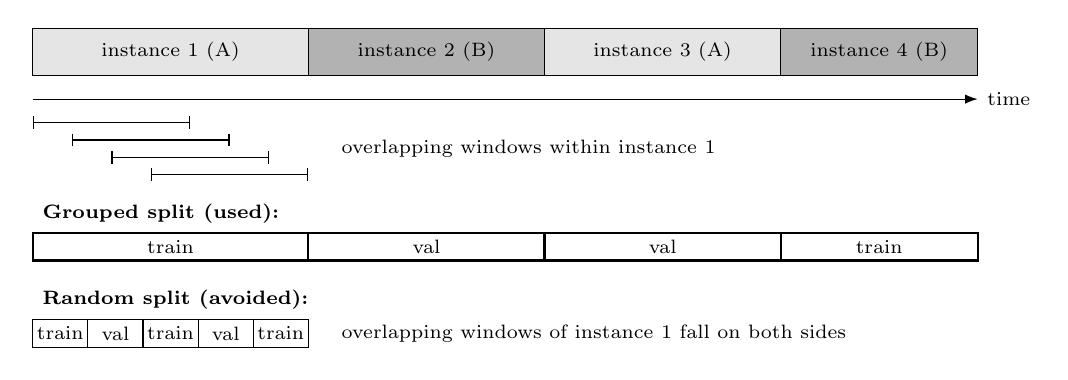
\begin{tikzpicture}[x=1cm, y=1cm, font=\scriptsize]
  % activity instances on the timeline
  \foreach \a/\b/\s/\t in {0/3.5/10/{instance 1 (A)}, 3.5/6.5/30/{instance 2 (B)},
                           6.5/9.5/10/{instance 3 (A)}, 9.5/12/30/{instance 4 (B)}} {
    \fill[black!\s] (\a,0) rectangle (\b,0.6);
    \draw (\a,0) rectangle (\b,0.6);
    \node at ({(\a+\b)/2},0.3) {\t};
  }
  \draw[-{Latex[length=1.6mm]}] (0,-0.3) -- (12,-0.3) node[right] {time};
  % overlapping windows of instance 1
  \foreach \i in {0,1,2,3} \draw[|-|] (0.5*\i,-0.6-0.22*\i) -- (0.5*\i+2,-0.6-0.22*\i);
  \node[anchor=west] at (3.8,-0.93) {overlapping windows within instance 1};
  % grouped assignment
  \node[anchor=west, font=\scriptsize\bfseries] at (0,-1.75) {Grouped split (used):};
  \foreach \a/\b/\s in {0/3.5/train, 3.5/6.5/val, 6.5/9.5/val, 9.5/12/train}
    \draw[thick] (\a,-2.35) rectangle (\b,-2.0) node[midway] {\s};
  % random assignment
  \node[anchor=west, font=\scriptsize\bfseries] at (0,-2.85) {Random split (avoided):};
  \foreach \i/\s in {0/train,1/val,2/train,3/val,4/train}
    \draw (0.7*\i,-3.45) rectangle (0.7*\i+0.7,-3.1) node[midway] {\s};
  \node[anchor=west] at (3.8,-3.28) {overlapping windows of instance 1 fall on both sides};
\end{tikzpicture}}
\caption{Grouped splitting. Overlapping windows are grouped into activity
instances, and whole instances are assigned to either the training or the
validation set. A random split would distribute the overlapping windows of one
instance across both sets.}
\label{fig:grouped-split}
\end{figure}

Table~\ref{tab:split} shows the resulting split. Because only whole groups can be
moved, the validation share of a class is not exactly 20\,\%. It exceeds the
target considerably when a class consists of a few long instances, as is the case
for \texttt{walk}, \texttt{measuring} and \texttt{place\_container}, where a single
group already contains a large part of the class. Overall, 946 windows (37\,\%)
fall into the validation set and 1619 windows (63\,\%) into the training set. For
\texttt{place\_container}, only 23 windows remain for training. This uneven split
is a consequence of keeping activity instances intact, and its effect on the
results is discussed in Chapter~\ref{ch:discussion}.

\begin{table}[htbp]
\centering
\small
\renewcommand{\arraystretch}{1.15}
\begin{tabular}{|l|r|r|r|r|}
\hline
\textbf{Class} & \textbf{Training} & \textbf{Validation} & \textbf{Total} & \textbf{Validation share} \\
\hline
\texttt{assemble\_parts}   & 130 &  36 & 166 & 22\,\% \\
\texttt{carry\_container}  & 175 &  45 & 220 & 20\,\% \\
\texttt{hammering}         & 170 &  80 & 250 & 32\,\% \\
\texttt{idle}              & 187 & 120 & 307 & 39\,\% \\
\texttt{insert\_screws}    & 185 &  61 & 246 & 25\,\% \\
\texttt{measuring}         & 159 & 161 & 320 & 50\,\% \\
\texttt{place\_container}  &  23 &  51 &  74 & 69\,\% \\
\texttt{screw\_tightening} & 454 & 142 & 596 & 24\,\% \\
\texttt{walk}              & 136 & 250 & 386 & 65\,\% \\
\hline
\textbf{Total}             & \textbf{1619} & \textbf{946} & \textbf{2565} & \textbf{37\,\%} \\
\hline
\end{tabular}
\caption{Training and validation windows per class after the grouped split.}
\label{tab:split}
\end{table}

\subsection{Metrics}
\label{sec:metrics}

Overall accuracy, the share of correctly classified validation windows, is used as
the main measure for comparing the models. Because the classes are imbalanced,
accuracy alone can hide poor performance on small classes. Precision, recall and
F1-score are therefore also reported for each class, together with the
macro-averaged F1-score, which gives every class the same weight {[}CITATION{]}. Confusion matrices are used to identify which activities are mistaken
for one another. Unless stated otherwise, all results are reported on the
validation set of the grouped split and come from a single training run per
model.

\section{Chapter Summary}
\label{sec:ch4-summary}

This chapter introduced the models compared in this thesis. Inertial windows are
processed as $200 \times 6$ time series by a 1D CNN, and audio windows as
$198 \times 40$ log-mel spectrograms by a 2D CNN, for which three pooling variants
were developed to make use of the temporal structure of the sounds. The two
modalities are combined at the input level (channel concatenation and unified
spectrogram), at the level of learned embeddings, and at the level of class
probabilities, where a per-class weighting reflects the different reliability of
the two modalities across activities. A random forest on hand-crafted features
serves as a classical baseline, and reduced, regularised variants prepare the
deployment on the device. All models share the same input normalisation, class
weighting, training settings, best-epoch selection and grouped train/validation
split. Chapter~\ref{ch:implementation} describes how selected models were
converted for execution on the wearable device, and Chapter~\ref{ch:results}
presents the results.
 % Load Data from File chapter4.tex (defines \label{ch:method})

\chapter{Results and Evaluation}
\label{ch:results}
% Chapter 5 -- to be written.

\chapter{Discussion}
\label{ch:discussion}
% Chapter 6 -- to be written.

\chapter{Conclusion}
\label{ch:conclusion}
% Chapter 7 -- to be written.

%---------------------------------------------------------
% bibliography based on Springer Design
%---------------------------------------------------------

\bibliographystyle{splncs03}
\bibliography{bibliography}

\printindex

\end{document}
